\documentclass{article}
\usepackage[utf8]{inputenc}
\usepackage{indentfirst}
\usepackage{titling}
\usepackage{geometry}
\usepackage{graphicx}
\graphicspath{ {./Images/} }
\usepackage[shortlabels]{enumitem}
\usepackage{fancyhdr}
\usepackage{ulem}
\usepackage[dvipsnames]{xcolor}
\usepackage{amssymb}
\usepackage{listings}
\usepackage{color}

\definecolor{dkgreen}{rgb}{0,0.6,0}
\definecolor{gray}{rgb}{0.5,0.5,0.5}
\definecolor{mauve}{rgb}{0.58,0,0.82}

\lstset{frame=tb,
  language=Java,
  aboveskip=3mm,
  belowskip=3mm,
  showstringspaces=false,
  columns=flexible,
  basicstyle={\small\ttfamily},
  numbers=none,
  numberstyle=\tiny\color{gray},
  keywordstyle=\color{blue},
  commentstyle=\color{dkgreen},
  stringstyle=\color{mauve},
  breaklines=true,
  breakatwhitespace=true,
  tabsize=3
}

\def\ojoin{\setbox0=\hbox{$\bowtie$}%
  \rule[-.02ex]{.25em}{.4pt}\llap{\rule[\ht0]{.25em}{.4pt}}}
\def\leftouterjoin{\mathbin{\ojoin\mkern-5.8mu\bowtie}}
\def\rightouterjoin{\mathbin{\bowtie\mkern-5.8mu\ojoin}}
\def\fullouterjoin{\mathbin{\ojoin\mkern-5.8mu\bowtie\mkern-5.8mu\ojoin}}

\renewcommand\maketitlehooka{\null\mbox{}\vfill} %para centralizar verticalmente
\renewcommand\maketitlehookd{\vfill\null}
\pagestyle{fancy}
\fancyhf{}
\rfoot{\thepage}
\lfoot{ 
\includegraphics[scale=0.01]{UA.jpg} José Mendes 107188 LEI}
\geometry{
  a4paper,
  headheight=4cm,
  top=5.5cm,
  bottom=4.5cm,
  footskip=4cm
}


\title{Segurança Informática e nas Organizações - Resumos 2}
\author{José Mendes 107188}
\date{2023/2024}

\begin{document}


\begin{titlepage}
    \maketitle
    \begin{center}
        
\includegraphics[scale=0.4]{UA.png}
    \end{center}
    \thispagestyle{empty} %remove o count da pagina
\end{titlepage}

\pagebreak

\section{Criptografia Assimétrica}

\subsection{Criptografia Assimétrica (de blocos)}

\begin{flushleft}
  \textbf{Usa um par de chaves:}
  \begin{itemize}
    \item \textbf{Chave privada:} pessoal, não transmissível;
    \item \textbf{Chave pública:} disponível a todos;
  \end{itemize}

  \vspace{2mm}

  \textbf{Permite:}
  \begin{itemize}
    \item Confidencialidade sem qualquer exchange of secrets prévia;
    \item Autenticação
    \begin{itemize}
      \item De conteúdos (integridade dos dados);
      \item De origem (atenticação da source, ou assinatura digital);
    \end{itemize}
  \end{itemize}
\end{flushleft}

\subsection{Operaçõees de uma Cifra Assimétrica}

\begin{center}
  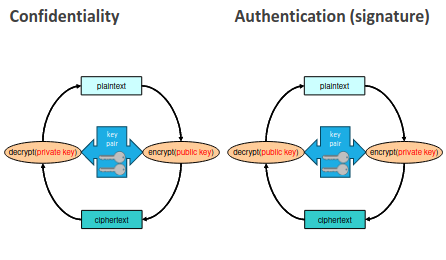
\includegraphics[scale=0.6]{1}
\end{center}

\subsection{Use Cases: Comunicação Segura}

\begin{flushleft}
  \textbf{Comunicação segura com um target (Bob)}
  \begin{itemize}
    \item A Alice encrípta o plaintext \textbf{P} com a chave pública do Bob, \textbf{Kpub\_Bob}
    \begin{itemize}
      \item \textbf{Alice: $C = \{P\}_{kpub\_bob}$}
    \end{itemize}
    \item O Bob decifra o ciphertext \textbf{C} com a sua chave privada, \textbf{Kpriv\_Bob}
    \begin{itemize}
      \item \textbf{Bob: $P' = \{C\}_{kpriv\_bob}$}
    \end{itemize}
    \item $P'$ deve ser igual a \textbf{P} (é necessário verificar)
    \item \textbf{Kpub\_Bob} precisa de ser conhecida pela Alice
  \end{itemize}
\end{flushleft}

\pagebreak

\begin{center}
  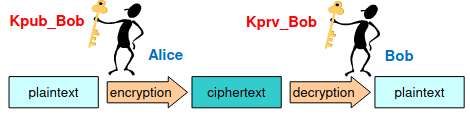
\includegraphics[scale=0.6]{2}
\end{center}

\subsection{Cifras Assimétricas}

\begin{flushleft}
  \textbf{Vantagens:}
  \begin{itemize}
    \item São um mecânismo de autenticação fundamental;
    \item Permitem explorar caracteristicas que não são possíveis com cifras simétricas;
  \end{itemize}

  \vspace{2mm}

  \textbf{Desvantagens:}
  \begin{itemize}
    \item Performance;
    \item Normalmente não são muito eficientes e consomem muita memória;
  \end{itemize}

  \vspace{2mm}
  \textbf{Problemas:}
  \begin{itemize}
    \item Distribuição confiável de chaves públicas;
    \item O lifetime do par de chaves é limitado;
  \end{itemize}

  \vspace{2mm}

  \textbf{Abordagens: problemas matemáticos complexos}
  \begin{itemize}
    \item Logaritmos discretos de números grandes;
    \item Factorização inteira de números grandes;
  \end{itemize}

  \vspace{2mm}
  \textbf{Algoritmos mais comuns:}
  \begin{itemize}
    \item RSA;
    \item ElGamal;
    \item Eliptic Curves (ECC);
  \end{itemize}

  \vspace{2mm}

  \textbf{Outras tecnicas com pares assimétricos de chaves:}
  \begin{itemize}
    \item Diffie-Hellman (key agreement);
  \end{itemize}
\end{flushleft}

\pagebreak

\subsection{RSA (Rivest, Shamir, Adelman, 1978)}

\begin{flushleft}
  \textbf{Chaves:}
  \begin{itemize}
    \item \textbf{Privada:} (d, n)
    \item \textbf{Pública:} (e, n)
  \end{itemize}

  \vspace{2mm}

  \textbf{Encriptação da chave pública (confidencialidade)}
  \begin{itemize}
    \item $C = P^e \hspace{2mm} mod \hspace{2mm} n$
    \item $P = C^d \hspace{2mm} mod \hspace{2mm} n$
  \end{itemize}

  \vspace{2mm}

  \textbf{Encriptação da chave privada (assinatura)}
  \begin{itemize}
    \item $C = P^d \hspace{2mm} mod \hspace{2mm} n$
    \item $P = C^e \hspace{2mm} mod \hspace{2mm} n$
  \end{itemize}

  \begin{center}
    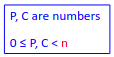
\includegraphics[scale=0.6]{3}
  \end{center}

  \textbf{Complexidade Computacional}
  \begin{itemize}
    \item Logaritmo discreto;
    \item Factorização inteira;
  \end{itemize}

  \vspace{2mm}

  \textbf{Seleção de Chaves}
  \begin{itemize}
    \item \textbf{n} grande (centenas ou milhares de bits);
    \item \textbf{$n = p \times q$} com \textbf{p} e \textbf{q} sendo números primos grandes (secretos);
    \item Escolher um \textbf{e} co-primo de \textbf{$(p-1) \times (q-1)$};
    \item Computar \textbf{d} tal que \textbf{$e \times d \equiv 1 \hspace{2mm} (mod \hspace{2mm} (p-1) \times (q-1))$};
    \item Discartar \textbf{p} e \textbf{q};
    \item O valor de \textbf{d} não pode ser facilmente computado a partir de \textbf{e} e \textbf{n} (apenas de \textbf{p} e \textbf{q});
  \end{itemize}
\end{flushleft}

\pagebreak

\subsubsection{RSA - Exemplo}

\begin{center}
  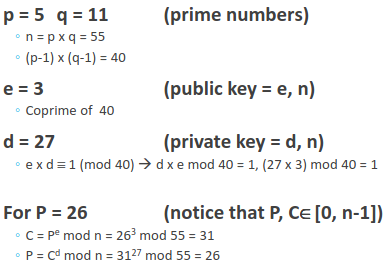
\includegraphics[scale=0.6]{4}
\end{center}

\subsection{Encriptação Hibrida}

\begin{flushleft}
  \textbf{Mistura criptografia simétrica com assimétrica}
  \begin{itemize}
    \item Usa o melhor dos dois mundos, evitando os problemas;
    \item Cifra assimétrica: usa chaves públicas (mas é lenta);
    \item Cifra simétrica: Rápida (mas com métodos fracos de troca de chaves);
  \end{itemize}

  \vspace{2mm}

  \textbf{Método}
  \begin{itemize}
    \item Obtém \textbf{$K_{pub}$} do destinatário;
    \item Gera uma chave simétrica aleatória \textbf{$K_{sym}$};
    \item Calcula \textbf{$C1 = E_{sym}(K_{sym}, P)$};
    \item Calcula \textbf{$C2 = E_{asym}(K_{pub}, K_{sym})$};
    \item Envia \textbf{$C1 + C2$};
    \begin{itemize}
      \item $C1$ é o texto encriptado com a chave simétrica;
      \item $C2$ é a chave simétrica encriptada com a chave pública do destinatário (pode também conter um IV);
    \end{itemize}
  \end{itemize}
\end{flushleft}

\subsection{Randomização de encriptações assimétricas}

\begin{flushleft}
  \textbf{Resultado de encriptações assimétricas não deterministico (não é prevísivel)}
  \begin{itemize}
    \item \textbf{N} encriptações do mesmo valor, com a mesma chave, deve produzir \textbf{N} resultados diferentes;
    \item \textbf{Objetivo:} Previnir a descoberta de valores encriptados através de tentativa e erro;
  \end{itemize}

  \vspace{2mm}

  \textbf{Abordagens:} Concatenação de um valor a encriptar com dois valores,
  um fixo (para controlo de integridade) e outro aleatório (para randomização);
\end{flushleft}

\subsubsection{OAEP (Optimal Asymmetric Encryption Padding)}

\begin{center}
  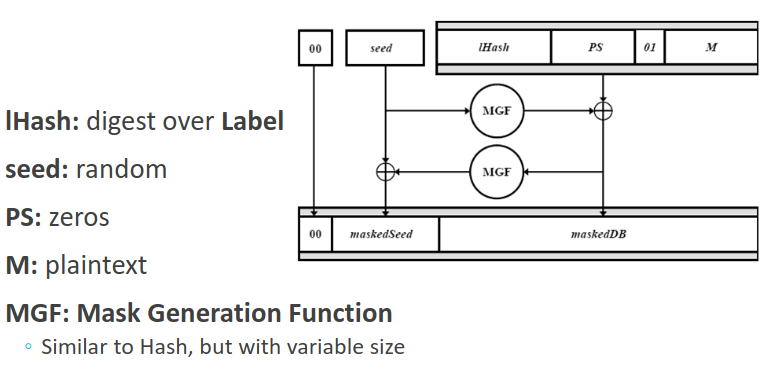
\includegraphics[scale=0.4]{5}
\end{center}

\subsection{Diffie-Hellman Key Agreement (1976)}

\begin{center}
  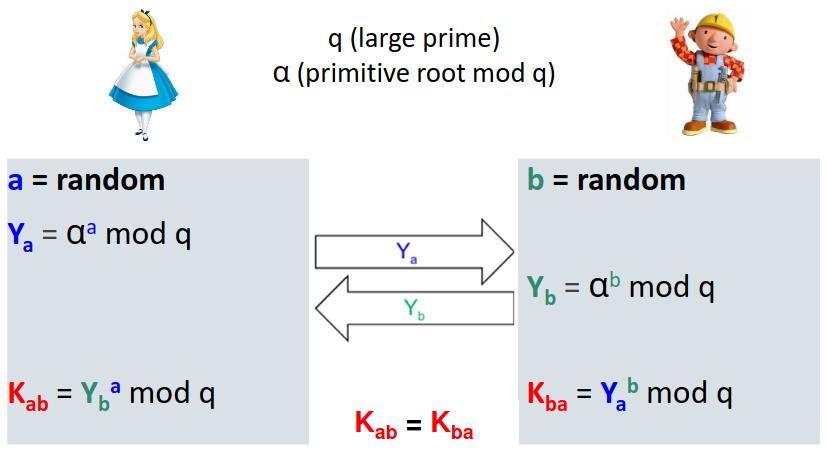
\includegraphics[scale=0.3]{6}
\end{center}

\subsubsection{DH Key Agreement: MitM Attack}

\begin{center}
  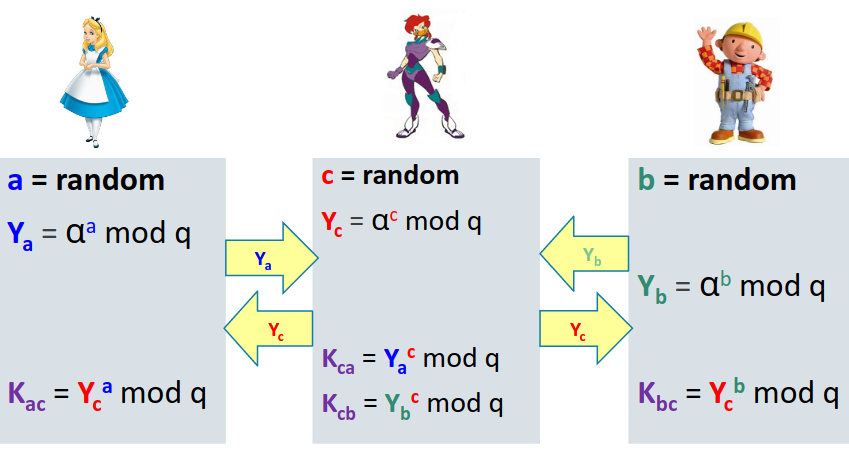
\includegraphics[scale=0.3]{7}
\end{center}

\pagebreak

\subsection{Eliptic Curve Cryptography (ECC)}

\begin{flushleft}
  \textbf{Curvas elipticas são funções específicas}
  \begin{itemize}
    \item Têm um gerador \textbf{G};
    \item Uma chave privada $K_{priv}$, é um inteiro com um máximo de
    bits permitidos pela curva;
    \item Uma chave pública $K_{pub}$, é um ponto $(x, y) = K_{priv} \times G$
    \item Dada $K_{pub}$, deve ser computacionalmente dificil determinar $K_{priv}$;
  \end{itemize}

  \begin{center}
    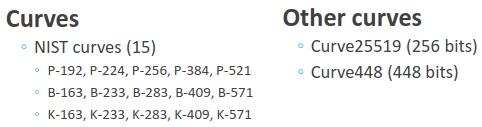
\includegraphics[scale=0.5]{9}
  \end{center}
\end{flushleft}

\subsection{ECDH: DH com ECC}

\begin{center}
  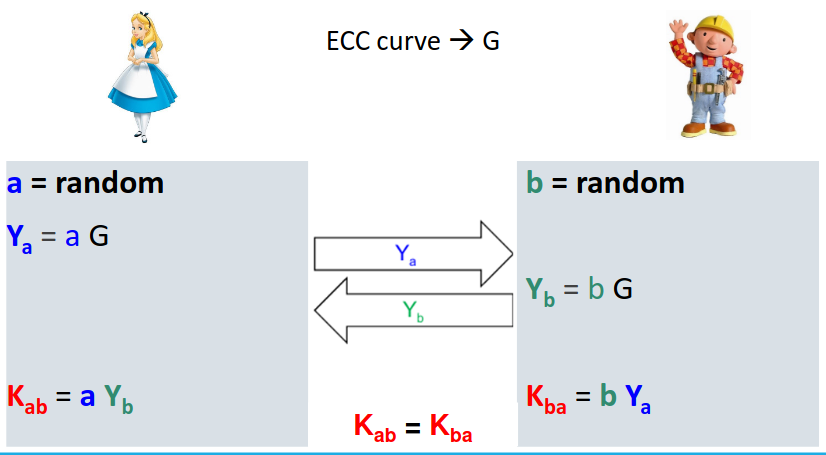
\includegraphics[scale=0.4]{8}
\end{center}

\subsection{Encriptação de chave pública com ECC}

\begin{flushleft}
  \textbf{Mistura encriptação hibrida com EDHC}

  \pagebreak

  \textbf{Método}
  \begin{itemize}
    \item Obtém $K_{pub\_recv}$ do destinatário;
    \item Gera um random $K_{priv\_send}$ com um correspondente $K_{pub\_send}$;
    \item Calcula $K_{sym} = K_{priv\_send} \times K_{pub\_recv}$;
    \item $C = E(P, K_{sym})$;
    \item Envia $C + K_{pub\_send}$;
    \vspace{2mm}
    \item Destinatário calcula $K_{sym} = K_{pub\_send} \times K_{priv\_recv}$;
    \item $P = D(C, K_{sym})$;
  \end{itemize}
\end{flushleft}

\section{Assinaturas digitais}

\subsection{Cifras Assimétricas (de blocos)}

\begin{flushleft}
  \textbf{Usa pares de chaves:}
  \begin{itemize}
    \item Uma \textbf{chave privada} (pessoal, não transmissível);
    \item Uma \textbf{chave pública} (disponível a todos);
  \end{itemize}

  \vspace{2mm}

  \textbf{Permite:}
  \begin{itemize}
    \item Confidencialidade sem qualquer exchange of secrets prévia;
    \item Autenticação
    \begin{itemize}
      \item De conteúdos (integridade dos dados);
      \item De origem (atenticação da source, ou assinatura digital);
    \end{itemize}
  \end{itemize}
\end{flushleft}

\subsection{Assinaturas Digitais}

\begin{center}
  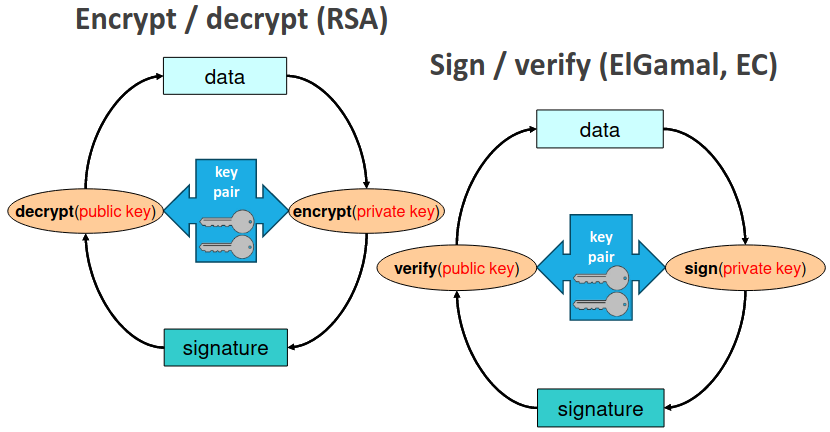
\includegraphics[scale=0.4]{10}
\end{center}

\pagebreak

\begin{flushleft}
  \textbf{Autenticação de conteúdos de um documento} - Garante a sua integridade
  (não se alterou);

  \vspace{2mm}

  \textbf{Autenticação do autor} - Garante que a identidade do criador/origem;

  \vspace{2mm}

  \textbf{Previnir repudiação de assinaturas}
  \begin{itemize}
    \item Non-repudiation (o autor não pode negar a autoria);
    \item Autores genuínos não podem negar a autoria (apenas a identidade
    do autor pode gerar uma dada assinatura);
  \end{itemize}

  \vspace{2mm}

  \textbf{Aboradgens}
  \begin{itemize}
    \item Encriptação/Decifração assimétrica ou assinatura/verificação;
    \item Funções digest (apenas para performance);
  \end{itemize}
\end{flushleft}

\begin{center}
  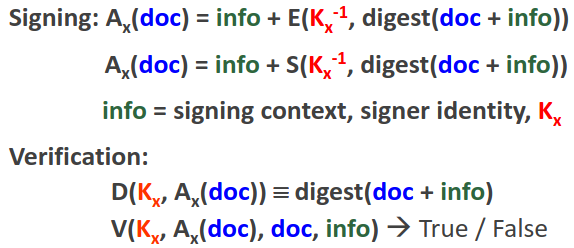
\includegraphics[scale=0.4]{11}
\end{center}

\subsubsection{Encriptação/Decifração signatures}

\begin{center}
  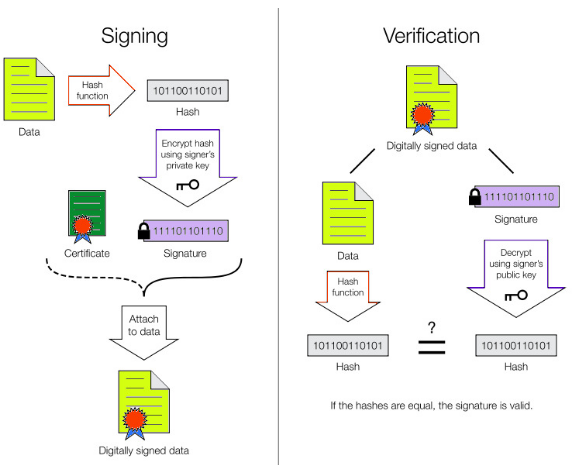
\includegraphics[scale=0.5]{12}
\end{center}

\pagebreak

\subsubsection{Assinatura digital num email: Multipart content, signature w/ certificate}

\begin{center}
  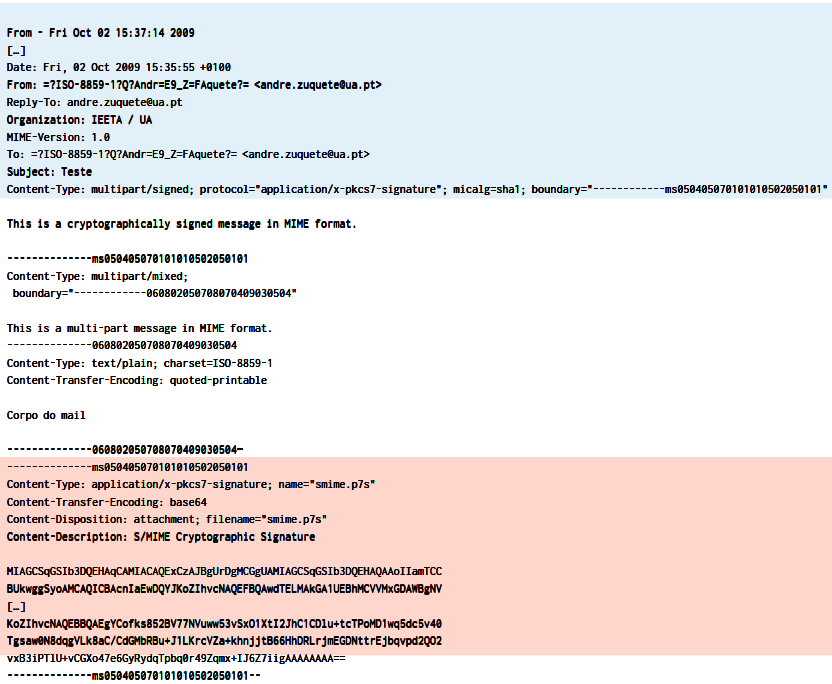
\includegraphics[scale=0.5]{13}
\end{center}

\pagebreak

\section{Derivação de chaves}

\begin{flushleft}
  \textbf{Algotitmos de cifras requerem chaves de tamanho fixo} - 56, 128, 256,\dots bits;

  \vspace{2mm}

  \textbf{Podemos derivar chaves de múltiplas origens}- shared secrets, passwords
  geradas por humanos, PIN codes e secrets de tamanho pequeno;

  \vspace{2mm}

  \textbf{Origem original pode ter baixa entropia} - reduz a dificuldade de
  ataques de força bruta, no entanto, devemos ter uma relação forte
  para uma chave útil;

  \vspace{2mm}

  \textbf{Por vezes percisamos de múltiplas chaves do mesmo material} -
  enquanto não permite encontrar o material (a password, outra chave)
  de uma chave nova;
\end{flushleft}

\subsection{Prepósitos de derivação de chaves}

\begin{flushleft}
  \textbf{Refroço de chaves: aumenta a segurança de uma password}
  \begin{itemize}
    \item Nomralmente definido por humanos;
    \item Tornando ataques de dicionário nada práticos;
  \end{itemize}

  \vspace{2mm}

  \textbf{Expansão de chaves: aumenta o tamanho de uma chave}
  \begin{itemize}
    \item Expande o tamanho que serve o algoritmo;
    \item Eventualmente deriva outras chaves relacionadas para outros algoritmos (ex: MAC);
  \end{itemize}
\end{flushleft}

\subsection{Derivação de chaves}

\begin{flushleft}
  \textbf{Derivação de chaves requer a existência de:}
  \begin{itemize}
    \item Um \textbf{salt} que trona a derivação única;
    \item Um problema difícil;
    \item Um nível de complexidade escolhido;
  \end{itemize}

  \vspace{2mm}

  \textbf{Dificuldade de Computação}
  \begin{itemize}
    \item A transformação requer recursos computacionais relevantes;
  \end{itemize}

  \vspace{2mm}

  \textbf{Dificuldade de Memória}
  \begin{itemize}
    \item A transformação requer recursos de armazenamento relevantes;
    \item Limita os ataques usando aceleração de hardware;
  \end{itemize}
\end{flushleft}

\pagebreak

\subsection{Derivação de chaves: PKBDF2}

\begin{flushleft}
  \textbf{Password Based Key Derivation Function 2}

  \vspace{2mm}

  \textbf{Produz uma chave a partir de uma password, com uma dificuldade escolhida}

  \[ K = PBKDF2(PRF, Salt, rounds, dim, password) \]

  \begin{itemize}
    \item \textbf{PRF} - Pseudo-Random-Function: função digest;
    \item \textbf{Salt} - Valor aleatório;
    \item \textbf{Rounds} - O custo computacional (dezenas ou centenas de milhares);
    \item \textbf{Dim} - Tamanho do resultado pretendido;
  \end{itemize}

  \vspace{2mm}

  \textbf{Operação: calcula operações ROUNDS x DIM a partir do PRF utilizando
  o SALT e a PASSWORD} - um tamanho maior de rounds aumenta a custo;
\end{flushleft}

\begin{center}
  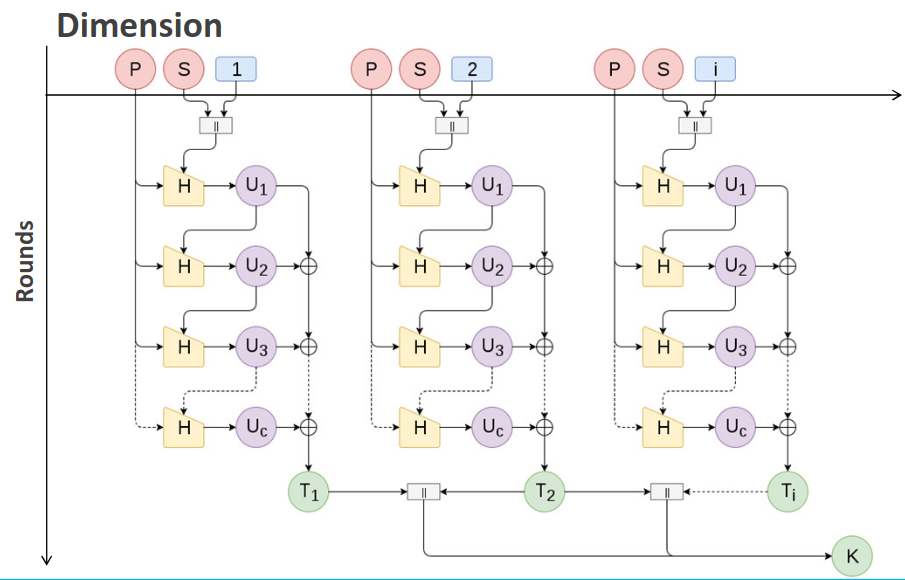
\includegraphics[scale=0.3]{14}
\end{center}

\pagebreak

\subsection{Derivação de chaves: Scrypt}

\begin{flushleft}
  \textbf{Produz uma chave com um custo de armazenamento escolhido}

  \vspace{2mm}

  \[ K = scrypt(password, salt, n, p, dim, r, hLen, Mflen) \]

  \begin{itemize}
    \item \textbf{Password} - Um segredo;
    \item \textbf{Salt} - Valor aleatório;
    \item \textbf{n} - Parâmetro de custo;
    \item \textbf{p} - Parâmetro de paralelismo $p \le (2^{32} -1) \times hLen / Mflen$;
    \item \textbf{dim} - Tamanho do resultado pretendido;
    \item \textbf{r} - Tamanho do bloco a usar (default: 8);
    \item \textbf{hLen} - Tamanho do da função digest (32 para SHA256);
    \item \textbf{Mflen} - Bytes na internal mix (default: $8 \times r$);
  \end{itemize}
\end{flushleft}

\begin{center}
  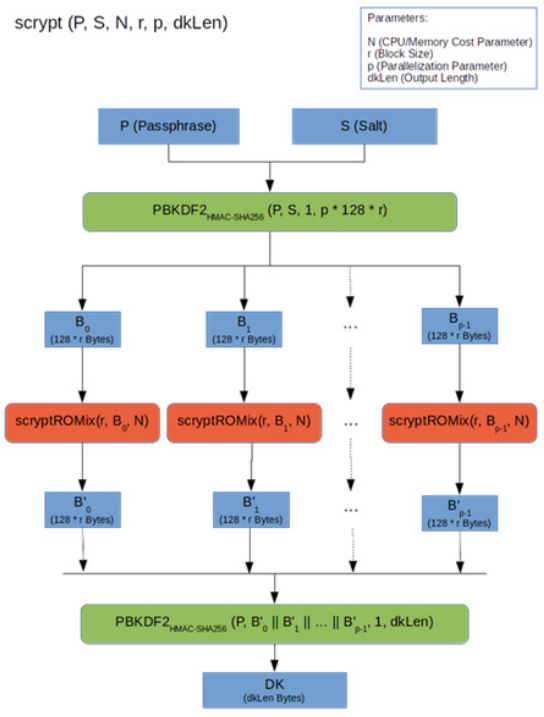
\includegraphics[scale=0.3]{15}
\end{center}

\pagebreak

\section{Gestão de chaves assimétricas}

\subsection{Problemas a resolver}

\begin{flushleft}
  \textbf{Garante um uso correto do par de chaves assimétricas}

  \begin{itemize}
     
  

    \item \textbf{Privacidade das chaves privadas}
    \begin{itemize}
      \item Garante a autenticidade;
      \item Previne a repudiação de assinaturas digitais;
    \end{itemize}

    \item \textbf{Distribuição correta de chaves públicas}
    \begin{itemize}
      \item Garante confidencialidade;
      \item Garante a correta validação de assinaturas digitais;
    \end{itemize}

  \end{itemize}

  \vspace{2mm}

  \textbf{Evolução temporal da entidade $\longleftrightarrow$ mapeamento de pares chave}

  \begin{itemize}
  
    \item \textbf{Para combater ocurrência catastróficas} (ex: perda de chaves privadas)

    \item \textbf{Para combater os requisitos de exploitations normais}
    (ex: refresh do par de chaves para reduzir riscos personificação)

  \end{itemize}

  \vspace{2mm}

  \textbf{Garante a correta geração de pares de chaves}
  \begin{itemize}
    \item \textbf{Geração aleatória de valores secretos}, de forma a poderem ser facilmente previstos;
    \item \textbf{Aumentar a eficiência sem reduzir a segurança}
    \begin{itemize}
      \item Tornar mecânismos de segurança mais eficientes;
      \item Aumentar a performance;
    \end{itemize}
  \end{itemize}
\end{flushleft}

\subsection{Objetivos}

\begin{flushleft}
  \begin{itemize}
    \item \textbf{Geração do par de chaves} - quando e como gerar;
    \item \textbf{Lidar com a chave privada} - como manter a chave privada;
    \item \textbf{Distribuição da chave pública} - como ditribuir corretamente as chaves públicas world-wide;
    \item \textbf{Tempo de vida do par de chaves} - quando vão expirar, até quando as usar e como verificar
    se esse par de chaves está obsuleto;
  \end{itemize}
\end{flushleft}

\pagebreak

\subsection{Geração de pares de chaves: Principais Designs}

\textbf{Usar bons geradores de números aleatórios para produzir segredos}

\begin{flushleft}
  \textbf{O resultado é indestinguível de noise}, isto é,
  todos os valores possíveis são igualmente prováveis e,
  não existem padrões resultantes do número da iteração ou de valores prévios;

  \vspace{2mm}

  \textbf{Exemplo: Bernoulli 1/2 Generator}
  \begin{itemize}
    \item Gerador sem memória;
    \item $P(b=1) = P(b=0) = 1/2$;
    \item Coin toss (atirar uma moeda ao ar);
  \end{itemize}
\end{flushleft}

\textbf{Facilidade sem comprometer a segurança}

\begin{flushleft}
  \textbf{Chaves públicas eficientes}
  \begin{itemize}
    \item Algumas são 1 bits, tipicamente $2k + 1$ valores (3, 17, 65537);
    \item Acelerar o processo com chaves públicas (o custo é proporcional ao número de bits 1);
    \item Sem security issues;
  \end{itemize}
\end{flushleft}

\textbf{Self-generation de chaves privadas}

\begin{flushleft}
  \textbf{Maximiza a privacidade, uma vez que outros nunca vão conseguir usar
  a dada chave privada}. Apenas o dono tem a chave, melhor ainda,
  o dono não tem a chave, mas pode usá-la;

  \vspace{2mm}

  \textbf{Principio pode ser relaxado quando não involve a geração de assinaturas}.
  Quando não existem issues relacionados com non-repudiation.
\end{flushleft}

\subsection{Lidar com chaves privadas}

\begin{itemize}
  \item \textbf{Correctness}
  
  \begin{itemize}
    \item \textbf{A chave privada representa o sujeito} (i.e., um cidadão, um servidor, etc.).
    O seu compromise deve ser minimizado. Cópias físicas seguras (backups) podem existir em alguns casos;

    \item \textbf{O caminho de acesso à chave privada deve ser controlado}.
    Proteção de acesso com password ou PIN code. Correctness das aplicações que usam;
  \end{itemize}

  \item \textbf{Confinement}
  \begin{itemize}
    \item \textbf{Proteção da chave privada dentro de um domínio seguro (reduzido) (ex: cryptographic token)}.
    O Token gera pares de chaves, exporta a chave pública mas nunca a privada, e, este Token
    encripta/decifra internamente com a chave privada.

    \item \textbf{Exemplo: SmartCards}, podemos pedir ao cartão para cifrar/decifrar
    algo. A chave privada nunca sai do SmartCard.
  \end{itemize}
\end{itemize}

\pagebreak

\subsection{Distribuição de chaves públicas}

\begin{flushleft}
  \textbf{Distribuição a todos os \uline{senders} de dados confidenciais}.
  Processo manual, usando um shared secret. Ad-hoc usando certificados digitais;

  \vspace{2mm}

  \textbf{Distribuição a todos os \uline{receivers} de assinaturas digitais}.
  Processo manual. Ad-hoc usando certificados digitais;
\end{flushleft}

\subsubsection{Problema}

\textbf{Como garantir a Correctness de uma chave pública?}

\vspace{2mm}

\textbf{Disseminação confiável de chaves públicas} - Paths/Graphs confiáveis.
Se \textbf{A confia em $K_X^+$} e \textbf{B confia em A}, então
\textbf{B confia em $K_X^+$}.

Hierarquias de certificação/grafos com as relações de confiança
expressas entre entidades. Certificação é unidirecional!

\subsection{Public key (digital) certificates}

É um \textbf{documento digital issued por uma autoridade de certificação (CA)}

\begin{itemize}
  \item \textbf{Liga a chave pública a uma entidade} (ex: pessoa, servidor ou serviço);
  \item \textbf{São documentos públicos}, não contêm informação privada,
  apenas pública. Pode ter informação adicional (ex: URL, nome, email, etc.);
  \item \textbf{São seguros criptograficamente},
  digitalmente assinados pelo issuer, não podem ser alterados;
\end{itemize}

\textbf{Pode ser usado para ditribuir chaves públicas de uma forma confiável}

\begin{flushleft}
  \textbf{O certificate receiver pode ser validade de várias formas}
  \begin{itemize}
    \item Com a chave pública do CA;
    \item Pode também validar a identificação;
    \item Validar a validade;
    \item Validar se a chave está a ser usada para o propósito correto;
  \end{itemize}

  \vspace{2mm}

  \textbf{O certificate receiver confia no comportamento do CA}, pelo que
  confia os documentos que este assina. Quando o CA associa um certificado a A,
  se o receicer confiar no CA, então confia que a associação de A é correta.
\end{flushleft}

\pagebreak

\begin{center}
  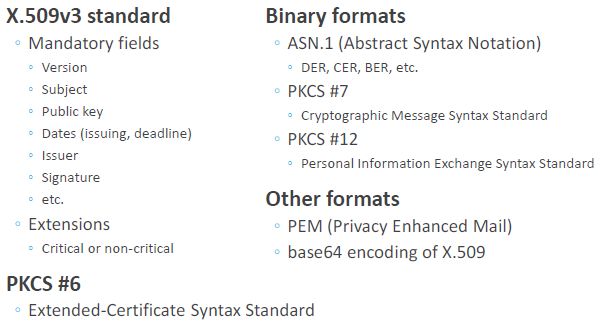
\includegraphics[scale=0.6]{16}
\end{center}

\subsection{Key pair usage}

\textbf{O certificado publico conecta o par de chaves a um perfil de utilização}.
As chaves privadas raramente são multifuncionais.

\vspace{2mm}

\textbf{Perfil de utilização tipico}
\begin{itemize}
  \item Autenticação/distribuição de chaves
  (Digital signature, Key encipherment, Data encipherment, Key agreement)
  \item Assinar documentos (Assinatura digital não repudiável)
  \item Certificate issuing (exclusivo de CAs). Assinar certificados,
  assinar CRLs (Certificate Revocation Lists)
  \item Timestamping (exclusivo de Time Stamping Authorities TSAs)
\end{itemize}

\textbf{Certificados de chaves públicas têm uma extensão para isto},
key usage (critical) que indica o perfil de utilização da chave pública.

\subsection{Assinatura de Certificados (CA)}

\begin{flushleft}
  \textbf{Organizações que gerem certificados de chaves públicas}.
  Companhias, não por lucro, governamentais, etc.;

  \vspace{2mm}

  \textbf{Define politicas e mecanismos para}:
  \begin{itemize}
    \item Issuing de certificados;
    \item Revoking de certificados;
    \item Distribuição de certificados;
    \item Issuing e distribuição das correspondentes chaves privadas;
  \end{itemize}

  \vspace{2mm}

  \textbf{Gerir a lista de certificados revogados} (CRLs), interfaces
  programaticas para verificar o estado atual de um certificado;
\end{flushleft}

\pagebreak

\subsection{Trusted Certification Authorities}

\begin{flushleft}
  \textbf{CAs intermediários} - CAs certificados por outras CAs confiaveis.
  Usando um certificado, permitindo a criação de uma hierarquia de certificação;

  \vspace{2mm}

  \textbf{Anchor confiavel (ou root CA)} - Um tem uma chave pública
  confiavel, normalmente implementada por certificados self-certified, ou seja,
  issuer e subject são o mesmo.

  Distribuição manual (ex: dentro do código do browser, OS, distribuição, etc.).
\end{flushleft}

Ver Exemplo de certificado nos slides 19-23.

\subsection{Refreshing of asymmetric key
pairs}

\begin{flushleft}
  \textbf{O par de chaves deve ter um tempo de vida limitado} - uma vez que,
  as chaves privadas podem ser perdidas ou descobertas, e para implementar
  uma politica de update;

  \vspace{2mm}

  \textbf{Problema} - Os certificados podem ser copiados e distribuidos.
  O universo de donos de certificados é desconhecido, pelo que, não podemos
  contactá-los para eliminar certificas específicos;

  \vspace{2mm}

  \textbf{Solução} - Certificados com um periodo de validade (nem antes, nem depois).
  Listas de certificados revogados, para revogar certificados
  antes da validade expirar;
\end{flushleft}

\subsection{Certificate Revocation Lists (CRLs)}

\begin{flushleft}
  \textbf{Base ou delta} - Completa / diferenças

  \vspace{2mm}

  \textbf{Listas de certificados assinados (identifiers) prematuramente
  invalidados} 
  \begin{itemize}
    \item Devem ser regularmente visitado por donos de certificados
    \item Protocolo OCSP para verificar a validade de um certificado (RFC 2560)
    \item Pode dizer a razão da revogação (slide 31)
  \end{itemize}

  \vspace{2mm}

  \textbf{Publicação e distribuição de CRLs} - Cada CA mantém
  a sua CRL e permite o acesso publico da mesma.
\end{flushleft}

\subsection{CRL e Delta CRL}

\begin{center}
  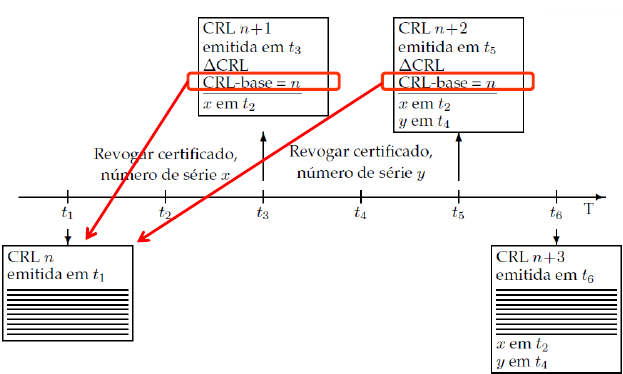
\includegraphics[scale=0.55]{17}
\end{center}

\pagebreak

\subsection{Online Certificate Status Protocol (OCSP)}

\begin{flushleft}
  \textbf{Protocolo baseado em HTTP para dar assert ao estado de um certificado}
  \begin{itemize}
    \item \textbf{Request} - Inclui o serial number do certificado;
    \item \textbf{Response} - Inclui se o certificado está revoked,
    é enviado pela CA e não possui validade;
    \item Uma verificação por certificado;
  \end{itemize}

  \vspace{2mm}

  \textbf{Requer menor largura de banda para clientes} -
  uma verificação por certificado em vez que fazer
  download de uma lista de certificados revogados (CRL);

  \vspace{2mm}

  \textbf{Involve maior largura de bannda para CAs} -
  uma verificação por certificado, problemas de privacidade
  uma vez que um CA saberá que um certificado está a ser usado;
  
  \vspace{2mm}

  \textbf{OOCSP stapling} - Inclui um timestamp recentemente assinado
  na resposta do servidor para dar assert à validade. Reduz a demora
  da verificação e carregamento no CA. Previne problemas de privacidade.
\end{flushleft}

\subsection{Distribuição de certificados de chaves públicas}

\begin{flushleft}
  \textbf{Transparente (integrado com sistemas ou aplicações)}
  \begin{itemize}
    \item Direcory systems, larga escala (ex: X.500 através de LDAP),
    organizacional (ex: Windows 2000 Active Directory), etc.;
    \item On-line: sem protocolos que usam certificados
    para autenticação peer (ex: protocolos de comunicação segura
    (TLS, IPSec, etc.), assinaturas digitais, dentro de MIME
    mail messages ou dentro de documentos);
  \end{itemize}

  \vspace{2mm}

  \textbf{Explicito (voluntáriamente ativado pelos users)}
  \begin{itemize}
    \item User faz request de um serviço para obter um certificado
    necessário (ex: pedido mandado por email, acesso a uma página HTTP pessoal).
  \end{itemize}
\end{flushleft}

\subsection{PKI (Public Key Infrastructure)}

\textbf{Infrastrutura para permitir um uso correto de chaves assimétricas e
de certificados de chave pública}.

\begin{flushleft}
  \textbf{Criação do par de chaves assimétricas para cada entidade que participa}.
  Politicas de participação, ploiticas de geração do par de chaves.

  \vspace{2mm}

  \textbf{Criação e distribuição de certificados de chaves públicas}.
  Politicas de participação, definição de atributos de certificados.

  \pagebreak

  \textbf{Definição e uso de certification chains (ou paths)}.
  Inserção numa hierarquia de certificação,
  certificação de outros CAs.

  \vspace{2mm}

  \textbf{Atualização, publicação e consulta de CRLs}.
  Politicas de revogação de certificados,
  serviços de distribuição de CRL, serviços OCSP.

  \vspace{2mm}

  \textbf{Usa estruturas de dados e protocolos permitindo inter-operabilidade
  entre componentes/serviços/pessoas}.
\end{flushleft}

\begin{center}
  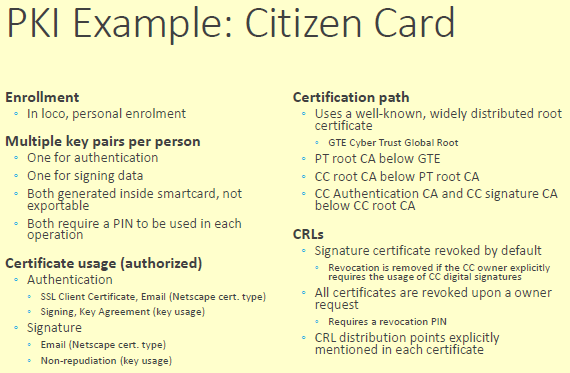
\includegraphics[scale=0.6]{18}
\end{center}

\subsection{Certificate Pinning}

\begin{flushleft}
  \textbf{Se um atacante tem acesso a uma Root confiavel, pode
  fingir ser qualquer entidade}. Manipula um CA confiavel
  em dar issue ao certificado (pouco provável).
  Injetar um CA costumizado na base de dados da vitima (mais provável).

  \vspace{2mm}

  \textbf{Certificate Pinning: adiciona a fingerprint do PubK (public key)
  ao \uline{código fonte}}. A fingerprint é uma hash (ex: SHA256).

  \vspace{2mm}

  \textbf{Validação do processo:} O certificado deve ser válido a regras locais,
  deve possuir uma chave pública com a dada fingerprint.
\end{flushleft}

\subsection{Certificate Transparency (RFC 6962)}

\begin{flushleft}
  \textbf{Problemas}
  \begin{itemize}
    \item CAs podem ser comprometidos (ex: DigiNotar) por atacantes,
    governo, etc.
    \item Comprometer é dificil de detetar. Resulta na mudança de
    suposições associadas com o comportamento do CA.
    O proprietário saberá sozinho.
  \end{itemize}

  \vspace{2mm}

  \textbf{Definição: um sistema global que regista todas as informações sobre
  certificados públicos criados}
  \begin{itemize}
    \item Garante que apenas um certificado tem as roots corretas;
    \item Guarda a chain de certificados inteira para cada certificado;
    \item Apresenta esta informação para auditoria (organizações
    ou ad-hoc por end users);
  \end{itemize}
\end{flushleft}

\pagebreak

\section{Mecanismos e Protocolos de Autenticação}

\subsection{Autenticação (Authn)}

\textbf{Prova de que uma entidade tem um atributo que diz ter}

\subsection{Authn: Tipos de Prova}

\begin{itemize}
  \item \textbf{Algo que a entidade sabe}: Um segredo memorizado (ou escrito \dots);
  \item \textbf{Algo que a entidade tem}: Um objeto/token apenas possuído pela entidade;
  \item \textbf{Algo que a entidade é}: A Biometria da entidade;
\end{itemize}

\subsubsection{Autenticação Multi-factor}

Usar simultaneamente diferentes tipos de prova. 2FA = Two Factor Authentication.

\subsubsection{Risk-based MFA}

MFA variável. Maior risco de ataque, mais fatores ou menos fatores risky.
Menor risco de ataque, menos fatores ou fatores mais simples.

\subsection{Authn: Objetivos}

\begin{itemize}
  \item \textbf{Autenticar interactors}, pessoas, serviços, servidores,
  hosts, redes, etc.;
  \item \textbf{Permitir o reforço das politicas e mecanismos de autorização},
  \begin{itemize}
    \item Autorização $\neq$ Autenticação;
    \item Autorização $\rightarrow$ Autenticação;
  \end{itemize}

  \item \textbf{Facilita o abuso (exploitation) de outros protocolos security-related}.
  Ex: distribuição de chaves para comunicação segura.
\end{itemize}

\subsection{Authn: Requisitos}

\begin{itemize}
  \item \textbf{Confiança (Trustworthiness)}
  \begin{itemize}
    \item Quão bom é em provar a identidade de uma entidade?
    \item Quão dificil é de ser enganada?
    \item Level of assurance (LoA) - Nível de confiança;
  \end{itemize}

  \item \textbf{Segredos (Secrecy)} - Nenhuma divulgação de credenciais secretas usadas por entidades legítimas.
\end{itemize}

\pagebreak

\begin{center}
  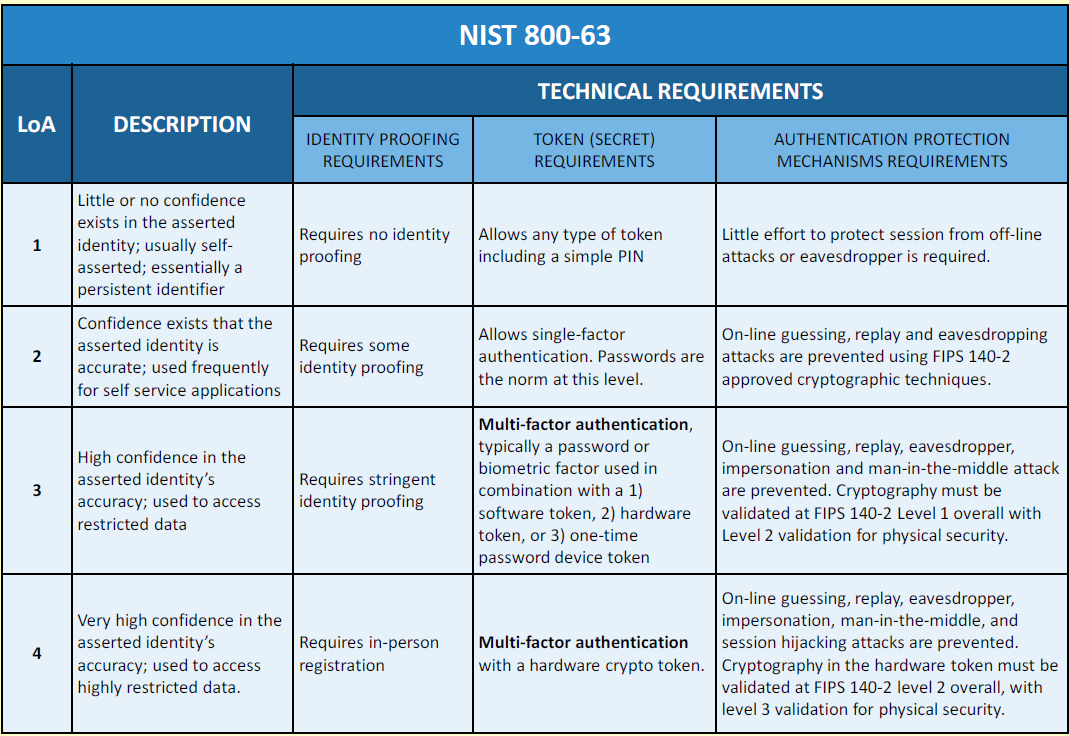
\includegraphics[scale=0.5]{19}
\end{center}

\begin{itemize}
  \item \textbf{Robustez (Robustness)}
  \begin{itemize}
    \item Previnir ataques ao protocolo de troca de dados;
    \item Previnir cenários de ataques on-line DoS;
    \item Previnir ataques de off-line dictionary;
  \end{itemize}

  \item \textbf{Simplicidade (Simplicity)} - Deve ser o mais simples
  possível para prevenir as entidades escolherem caminhos alternativos perigosos.

  \item \textbf{Lidar com vulnerabilidades introduzidas por pessoas}
  \begin{itemize}
    \item Têm uma tendencia natural a facilitar ou escolher atalhos;
    \item Lidar com phishing;
  \end{itemize}
\end{itemize}

\subsection{Authn: Entidades e Modelo de Deployment}

\vspace{2mm}

\begin{center}
  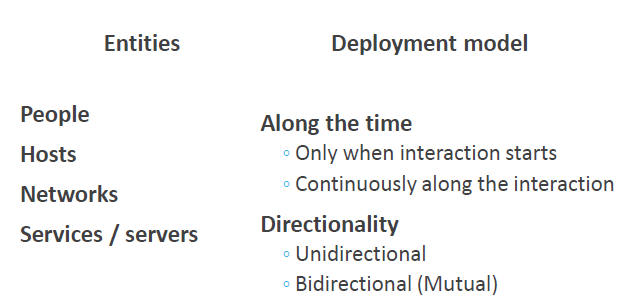
\includegraphics[scale=0.55]{20}
\end{center}

\pagebreak

\subsection{Authn interactions: Aboradgens Básicas}

\begin{flushleft}
  \textbf{Abordagem Direta}
  \begin{itemize}
    \item Fornecer credenciais;
    \item Esperar o veredito;
  \end{itemize}
  A \uline{vantagem} desta abordagem: \textbf{não é preciso computação} por parte do presenter.
  A \uline{desvantagem}: as credenciais podem ser \textbf{expostas} a validadores maliciosos.

  \vspace{2mm}

  \textbf{Abordagem Challenge-Response}
  \begin{itemize}
    \item Obter o desafio;
    \item Fornecer uma resposta computada a partir do desafio e das credenciais;
    \item Esperar o veredito;
  \end{itemize}
  A \uline{vantagem} desta abordagem: as credenciais \textbf{não são expostas} a validadores maliciosos.
  A \uline{desvantagem}: requere \textbf{computação} por parte do presenter.
\end{flushleft}

\subsection{Authn of subjects: Direct Approach w/ known password}

\textbf{Uma password é verificada comparando com valores previamnete armazenados},
para uma dada identidade (ex: username).

\vspace{2mm}

\textbf{Valor pessoal armazenado}: É transformado por uma função unidirecional.
Em Windows, uma digest function, em UNIX, DES hash + salt, em Linux,
MD5 + salt (hash é configurável).

\vspace{3mm}

\textbf{Melhor: PBKDF2, Script with high complexity}.

\begin{center}
  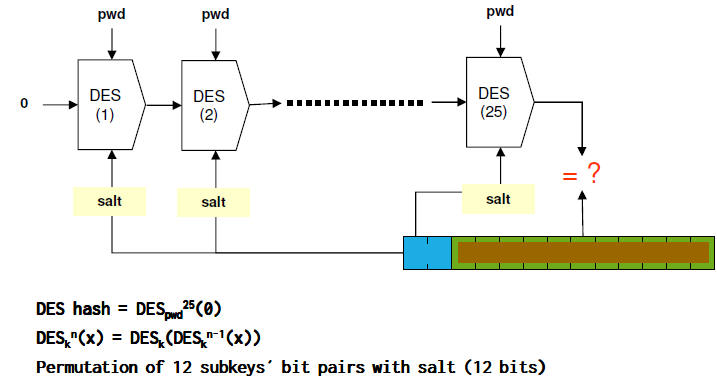
\includegraphics[scale=0.55]{21}
\end{center}

\begin{flushleft}
  \textbf{Vantagem:} Simplicidade;

  \vspace{2mm}

  \textbf{Problemas:} 
  
  \begin{itemize}
    \item A utilização de passwords fracas (permitindo dictionary attacks)
    \item Transmissão da password atraves de canais de comunicação inseguros,
    Eavesdroppers podem obter a password facilemnete (ex: Unix remote services, PAP);
  \end{itemize}
\end{flushleft}

\pagebreak

\subsection{Authn of people: Direct Approach w/ biometrics}

\begin{flushleft}
  \textbf{As pessoas são autenticadas usando partes do corpo}, como
  \uline{biometric samples}, fingerprints, iris, face geometry,
  voice timber, manual writing, vein matching, etc.

  \vspace{2mm}

  \textbf{Estas medidas são comparadas com registos pessoais} (referencias biometricas (templates)),
  registadas no sistema com um procedimento prévio de enrollment.

  \vspace{2mm}

  \textbf{Identificação vs Autenticação}
  \begin{itemize}
    \item \textbf{Identificação} - 1-to-many verificações para match;
    \item \textbf{Autenticação} - 1-to-1 verificações para match;
  \end{itemize}
\end{flushleft}

\begin{flushleft}
  \textbf{Vantagens:}
  \begin{itemize}
    \item As pessoas não precisam de memorizar ou ter a password consigo;
    \item As pessoas não podem escolher passwords fracas;
    \item As credenciais de autenticação não podem ser transferidas a outros;
  \end{itemize}

  \vspace{2mm}

  \textbf{Problemas:}
  \begin{itemize}
    \item Métodos biométricos ainda são pouco fiáveis, em muitos casos
    podem ser enganados facilmente (ex: fingerprint, face recognition, etc.);

    \item As pessoas não podem mostrar as credenciais (em caso de roubo);
    \item Credenciais não podem ser transferidas entre individuos (casos extraordiários);
    \item Podem causar perigos a inidivuos, a integridade física pode ser comprometida para obter as credenciais;
    \item Não é facil de ser implementada em sistemas remotos, pois é obrigatório ter dispositivos biométricos seguros e confiaveis;
    \item Biometrias podem revelar segredos de outras pessoas (doenças);
  \end{itemize}
\end{flushleft}

\subsection{Authn of subjects: Direct Approach w/ one-time passwords}

\begin{flushleft}
  \textbf{One-Time passwords = segredos que podem ser usados apenas uma vez}, pre-distribuidos diretamente,
  ou o resultado de uma função geradora. Exemplo: Códigos do banco, Google Backup Codes, etc.


  \vspace{2mm}

  \textbf{Vantagens:}
  \begin{itemize}
    \item Podem ser eavesdropped, permitindo o seu uso em canais sem encriptação;
    \item Podem ser escolhidas pelo authenticator, o que pode colocar uma dada complexidade;
    \item Pode depender de uma password partilhada;
  \end{itemize}

  \vspace{2mm}

  \textbf{Problemas:}
  \begin{itemize}
    \item Entidades a interagir precisam de saber qual password usar em cada ocasião;
    \item Individuos podem querer recursos adicionais para guardar/gerar passwords;
  \end{itemize}
\end{flushleft}

\pagebreak

\subsubsection{YubiKey}

\begin{flushleft}
  \textbf{Dispositivo pessoal de autenticação}: USB, Bluetooth e/ou NFC.

  \vspace{2mm}

  \textbf{Ativação gera uma chave de 44 caracteres}, emula um teclado USB, suporta HOTP (events) ou TOTP (temporal).
  Se um desafio é fornecido, o user toca no botão e obtem a resposta. Possui vários algorimos, incluindo AES 256.
\end{flushleft}

\begin{center}
  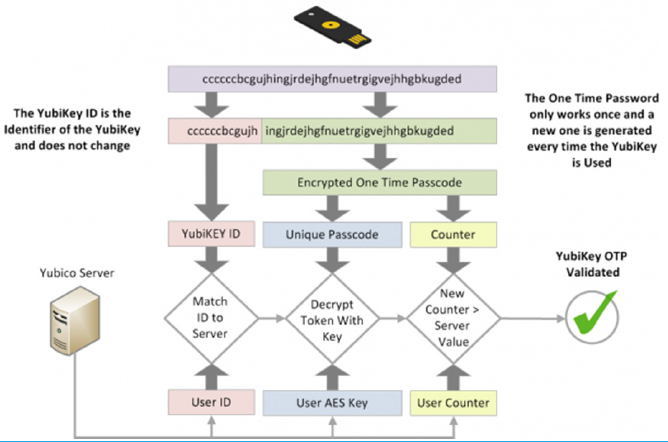
\includegraphics[scale=0.5]{22}
\end{center}

\subsection{Challenge-Response Approach}

\begin{flushleft}
  \textbf{O authenticator fornece um desafio}, um nonce (value not once used), normalmente random, pode ser um contador.

  \vspace{2mm}

  \textbf{A entidade autenticada transforma o desafio}, o método de transformação é partilhado pelo authenticator.

  \vspace{2mm}

  \textbf{O resultado é enviado de volta ao authenticator}

  \vspace{2mm}

  \textbf{O authenticator verifica o resultado}. Calcula o resultado utilizando
  o mesmo método e desafio, ou produz um valor do resultado e avalia se é igual
  ao desafio, ou a algum valor relacionado.

  \vspace{2mm}

  \textbf{Vantagens:}
  \begin{itemize}
    \item As credenciais de autenticação não são expostas;
    \item Um Eavesdropper vai ver o desafio e a resposta, mas não consegue
    calcular a resposta sem o método de transformação;
  \end{itemize}

  \pagebreak

  \textbf{Problemas:}

  \begin{itemize}
    \item Entidades autenticadas devem ter a capacidade de calcular resultados de desafios
    (hardware token ou software application);
    \item O authenticator deve precisar de manyer segredos partilhados (em clear text). Estes
    podem ser roubados, os users podem reutilizar segredos noutro sistema, permitindo ataques;
    \item Pode ser possível calcular todos os resultados para um (ou todos) desafio(s) (revelando o segredo usado);
    \item Pode ser vulneravel a dictionary attacks;
    \item O authenticator NUNCA deve enviar um mesmo desafio a um mesmo user;
  \end{itemize}
\end{flushleft}

\subsection{Authn of subjects: Challenge-Response w/ Smartcards}

\begin{flushleft}
  \textbf{Credenciais de autenticação}:
  \begin{itemize}
    \item Ter um smartcard (ex: cartão de cidadão);
    \item A chave privada guardada no smartcard;
    \item O PIN de acesso à chave;
  \end{itemize}

  \textbf{O authenticator sabe} a chave pública;

  \vspace{2mm}

  \textbf{Robusto contra:}
  \begin{itemize}
    \item Dictionary attacks;
    \item Ataque offlince a uma base de dados;
    \item Canais inseguros;
  \end{itemize}

  \vspace{2mm}

  \textbf{Prorocolo Challenge-Response}:
  \begin{itemize}
    \item O authenticator gera o desafio;
    \item O dono do smartcard cifra o desafio com a chave privada
    (guardada no smartcard, protegida pelo PIN). Em alternativa pode assinar o desafio;
    \item O authenticator decifra o resultado com a chave pública.
    Se o resultado da decifra corresponder ao desafio, a autenticação é bem sucedida. Em alternativa,
    pode verificar a assinatura (que é o mesmo processo);
  \end{itemize}
\end{flushleft}

\pagebreak

\subsection{Authn of subjects: Challenge-Response w/ Other Tokens}

\begin{flushleft}
  \textbf{Tokens FIDO2 (FIDO Alliance)}
  \begin{itemize}
    \item Para ambientes desktop e mobile;
    \item WebAuthn, especificação para web authentication;
    \item Client-to-Authenticator Protocol (CTAP);
    \item Segurança
    \begin{itemize}
      \item Credenciais nunca deixam o dispositivo do user e unca são guardadas num servidor;
      \item Sem risco de phishing, sem roubo de passwords (mesmo assim, o token pode ser roubado);
      \item Sem ataques de replay;
      \item Token certification levels;
    \end{itemize}
    \item Privacidade
    \begin{itemize}
      \item Credenciais são únicas por website;
      \item Tracking não é ppossivel (diferentes web sites, diferentes chaves públicas para um mesmo token);
      \item Dados biométricos, quando usados, nunca saem do dispositivo do user;
    \end{itemize}
  \end{itemize}
\end{flushleft}

\begin{center}
  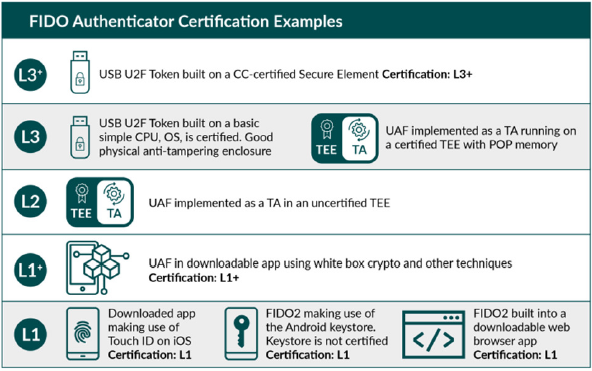
\includegraphics[scale=0.6]{23}
\end{center}

\subsection{Authn of subjects: Challenge-Response w/ Shared Secret}

\begin{flushleft}
  \textbf{Credenciais de autenticação}: Password selecionada pelo user;

  \vspace{2mm}

  \textbf{O authenticator sabe}:
  \begin{itemize}
    \item Péssima abordagem: a shared password;
    \item Melhor abordagem: Uma transformação da shared password.
    A transformação deve ser unidirecional;
  \end{itemize}

  \pagebreak

  \textbf{Protocolo Básico Challenge-Response}:

  \begin{center}
    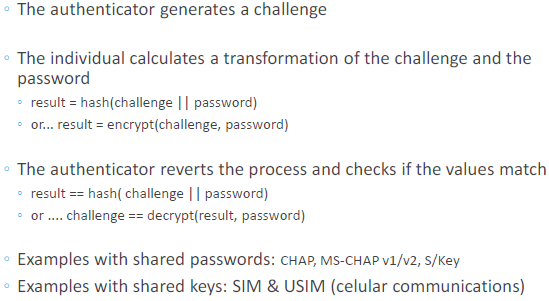
\includegraphics[scale=0.6]{24}
  \end{center}
\end{flushleft}

\subsection{PAP e CHAP (RFC 1334, 1992, RFC 1994, 1996)}

\begin{flushleft}
  \textbf{Protocolos utilizados para PPP (Point-to-Point Protocol)}.
  Autenticação unidirecional. O authenticator autentica users, \uline{mas
  os users não autenticam o authenticator}.

  \vspace{2mm}

  \textbf{PAP (PPP Authentication Protocol)}: Representação simples de um par de UID/password.
  Transmissão insegura (em clear text).

  \vspace{2mm}

  \textbf{CHAP (Challenge-response Authentication Protocol)}:
  \begin{itemize}
    \item Aut $\rightarrow$ U: authID, challenge;
    \item U $\rightarrow$ Aut: authID, MD5(authID, secret, challenge), identity;
    \item Aut $\rightarrow$ U: authID, OK/NOT OK;
  \end{itemize}

  O authenticator pode pedir mais autenticações a qualquer momento.
\end{flushleft}

\subsection{Authn of subjects: Challenge-Response w/ Shared Key}

\begin{flushleft}
  \textbf{Utiliza uma chave criptografica em vez de uma password}.
  Robusto contra dictionary attacks. Requer um dispositivo para
  armazenar a shared key.
\end{flushleft}

\subsection{GSM Subscriber Authentication}

\begin{flushleft}
  \textbf{Usa um segredo partilhado entre o HLR e o telemovel subscrito}
  \begin{itemize}
    \item Utiliza uma shared key de 128-bit (não é um par de chaves assimétricas);
    \item A chave é armazenada no SIM card;
    \item o SIM card é desbloqueado com um PIN;
    \item O SIM card responde a desafios usando a shared key;
  \end{itemize}

  \textbf{Utiliza (initially unkonwn algorithms):} A3 (autenticação),
  A8 (geração de session key), A5 (stream cipher para comunicação).

  \vspace{2mm}

  \textbf{A3 e A8 são executados pelo SIM, A5 é executado pela baseband}.
  A3 e A8 podem ser escolhidos pelo operador.
\end{flushleft}

\pagebreak

\begin{center}
  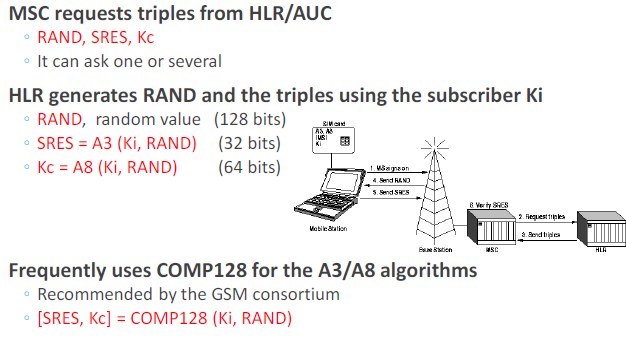
\includegraphics[scale=0.6]{25}
\end{center}

\subsection{Autenticação de Sistemas}

\begin{flushleft}
  \textbf{Por nome (DNS) ou MAC/IP address}: Muito fraco, sem prova
  criptografica. Mesmo assim é usado em alguns serviços (ex: NFS, TCP wrappers).

  \vspace{2mm}

  \textbf{Com chaves criptograficas}: Secret keys partilhadas entre entidades que
  comunicam frequentemente. Par assimétrico de chaves, um por host.
  Chaves públicas pre-partilhadas com entidades que comunicam frequentemente.
  Chaves públicas certificadas por umas third-party (um CA).

  \vspace{2mm}

  \textbf{Autenticação de um host}: Todos os serviços co-localizados num mesmo
  host são automaticamente e indiretamente autenticados.

  \vspace{2mm}

  \textbf{Credenciais exclusivas para cada serviço}

  \vspace{2mm}

  \textbf{Autenticação}:
  \begin{itemize}
    \item Secret keys partilhadas com clientes (quando estas precisam
    de autenticação dos clientes);
    \item Par de chaves assimétricas por host/service (certificado por outros ou não);
  \end{itemize}
\end{flushleft}

\subsection{TLS (Transport Layer Security, RFC 2246)}

\begin{flushleft}
  \textbf{Protocolo de segurança para comunicação em TCP/IP}.
  Evoluiu do SSL V3 (Secure Socket Layer). Gere sessões seguras sobre
  TCP/IP, individuais a cada aplicação. Inicialmente usado para o trafego
  de HTTP.

  \vspace{2mm}

  \textbf{Mecanismos de segurança}:
  \begin{itemize}
    \item Confidencialidade e integridade da comunicação entre entidades
    (distribuição de chaves, negociação de cifras, digests e outros mecanismos);
    \item Autenticação das entidades envolvidas
    \begin{itemize}
      \item Servers, serviços, etc.
      \item Clients (não tão comum)
      \item Ambos utilizando chaves assimétricas e certificados X.509;
    \end{itemize}
  \end{itemize}
\end{flushleft}

\pagebreak

\begin{center}
  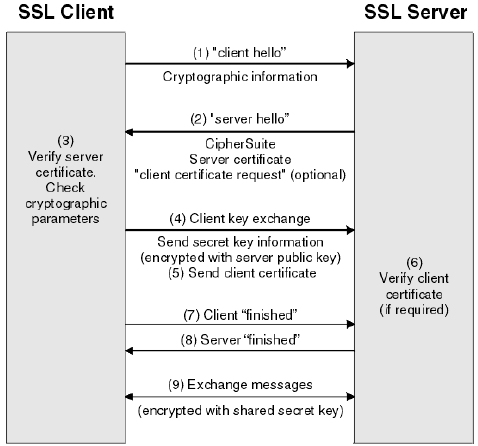
\includegraphics[scale=0.6]{26}
\end{center}

\subsection{TLS Ciphersuites}

\begin{flushleft}
  \textbf{Se um servidor suporta um único algoritmo, não pode experar que
  todos os clientes suportem o mesmo algoritmo} (mais poderoso/limitado, velho/novo).

  \vspace{2mm}

  \textbf{O conceito de ciphersuite permite a negociação de mecanismos
  entre cliente e servidor}. Ambos mandam os seus ciphersuites suportados,
  e escolhem um que ambos suportem. O servidor escolhe no caso.

  \vspace{2mm}

  \textbf{Exemplo:} ECDHE-RSA-AES128-GCM-SHA256

  \begin{itemize}
    \item \textbf{ECDHE} - Ephemeral Elliptic Curve Diffie-Hellman, é o algoritmo de negociação
    \item \textbf{RSA} - Algoritmo de autenticação;
    \item \textbf{AES-128 GCM} - Algoritmo de cifra e modo de cifra
    \item \textbf{SHA256} - Algoritmo de controlo de integridade
  \end{itemize}
\end{flushleft}

\subsection{SSH (Secure SHell)}

\begin{flushleft}
  \textbf{Gere sessões seguras da consola sobre TCP/IP}. Inicialmente desenhado
  para substituir o Telnet application/protocol. Atualmente utilizado
  em muitas outras aplicações\begin{itemize}
    \item Execução de comandos remotos de forma segura (rsh/rexec);
    \item Cópia segura de conteudos de/para hosts remotos (rcp);
    \item Transferência segura de ficheiros (sftp) (Secure FTP);
    \item Secure (Generic) communication tunnels (carry standard IP packets);
  \end{itemize}

  \pagebreak

  \textbf{Mecanismos de segurança}:
  \begin{itemize}
    \item Confidencialidade e integridade das comunicações (distribuição de chaves);
    \item Autenticação das entidades envolvidas
    \begin{itemize}
      \item Servidor/Hosts;
      \item Users;
      \item Os dois atingidos através de vários mecanismos diferenciados;
    \end{itemize}
  \end{itemize}
\end{flushleft}

\subsection{SSH: Mecanismos de Autenticação}

\begin{flushleft}
  \textbf{Servidor: Par de chaves assimétricas}
  \begin{itemize}
    \item As chaves são distribuidas durante a interação (not certified!);
    \item Os clientes guardam as chaves públicas de interações previas.
    A chave deve ser guardada em ambientes confiados. Se a chave mudar o cliente
    deve ser avisado (ex: servidor reinstalado, key regenerou, etc.).
  \end{itemize}

  \vspace{2mm}

  \textbf{Clientes: Autenticação é configuravel}
  \begin{itemize}
    \item Default: username + password;
    \item Outra: username + chave privada (a pública deve estar pré-instalada no servidor);
    \item Outra: itegração com PAM para mecanismos de autenticação alternativos;
  \end{itemize}
\end{flushleft}

\subsection{Centralized network authentication}

\begin{flushleft}
  \textbf{Usada para restringir o acesso à rede a clientes conhecidos}
  \begin{itemize}
    \item Redes de cabo;
    \item Redes wireless;
    \item Em VPNs (Virtual Private Networks);
  \end{itemize}

  \vspace{2mm}

  \textbf{Geralmente implementado por um serviço central}
  \begin{itemize}
    \item Servidor AAA (Authentication, Authorization, Accounting), ex: RADIUS e DIAMETER;
    \item O servidor define quais serviços de rede o user pode usar;
  \end{itemize}
\end{flushleft}

\pagebreak

\subsection{Autenticação por um IdP}

\begin{center}
  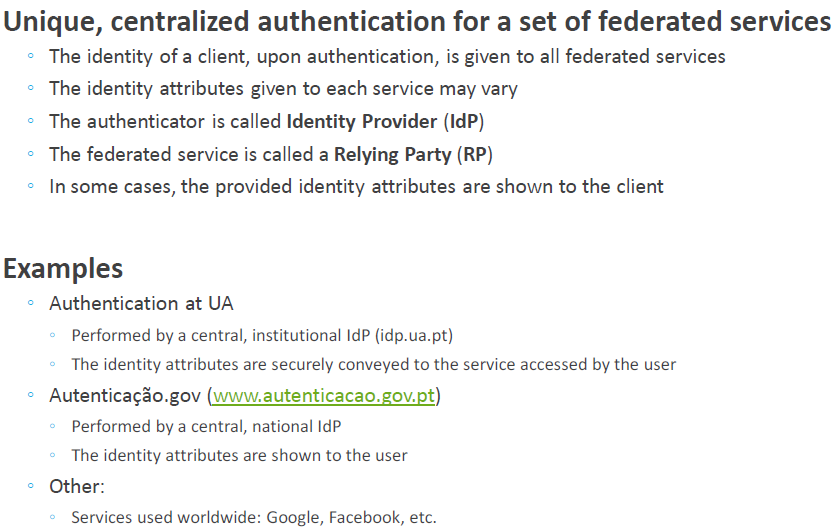
\includegraphics[scale=0.5]{27}
\end{center}

\subsection{Autenticação Centralizada}

\begin{flushleft}
  \textbf{Vantagens:}
  \begin{itemize}
    \item Pode reutilizar as mesmas credenciais sobre múltiplos sistemas/serviços;
    \item Repositório único e seguro para as credenciais (mais dificil de roubar Credenciais
    quando utilizado em varios serviços);
    \item Pode implementar restrições para serviços/sistemas;
  \end{itemize}

  \vspace{2mm}

  \textbf{Desvantagens:}
  \begin{itemize}
    \item Requer servidores adicionais;
    \item Single point of failure: sem sistemas de autenticação, ninguém
    pode ser autenticado (importante deploy a credenciais para admins);
    \item Introduz delays no processo de autenticação;
  \end{itemize}
\end{flushleft}

\subsection{Single Sign-On}

\begin{flushleft}
  \textbf{Uma facilidade normalmente associada com IdP}. Ambos
  não obrigatório e nem sempre apropriado.

  \vspace{2mm}

  \textbf{SSO existe para simplificar a vida dos users}. Eles fazem login
  apenas uma vez para acessar vários serviços durante um periodo de tempo.
\end{flushleft}

\pagebreak

\subsection{OAuth 2.0: delegação (RFC 6749)}

\begin{flushleft}
  \textbf{Uma framework para permitir aos users delegar acesso aos
  seus recursos pela sua conta}.
\end{flushleft}

\begin{center}
  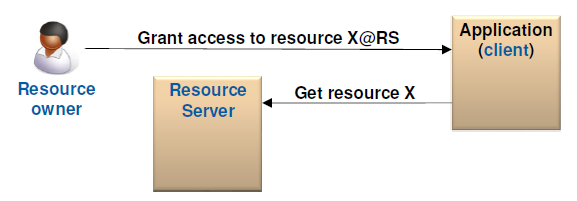
\includegraphics[scale=0.6]{28}
\end{center}

\subsection{OAuth 2.0 roles}

\begin{flushleft}
  \textbf{Resource Owner}: Uma entidade capaz de conceder acesso
  a um \textbf{recurso protegido}. \textbf{End-user}: um
  Resource Owner que é uma pessoa.

  \vspace{2mm}

  \textbf{Resource Server}: O servidor que hospeda os recursos protegidos.
  Responde a pedidos de acesso a recursos protegidos utilizando \textbf{tokens de acesso}.

  \vspace{2mm}

  \textbf{Client}: Uma \textbf{aplicação} que realiza requests por recursos protegidos
  em nome do Resource Owner e com a sua autorização.

  \vspace{2mm}

  \textbf{Authorization Server}: O servidor que emite tokens de acesso
  para os clientes após \textbf{autenticar o Resource Owner} com sucesso
  e obter a sua \textbf{autorização} para os clientes acederem a um dos seus
  (users) recursos.
\end{flushleft}

\subsection{Protocol Flow}

\begin{center}
  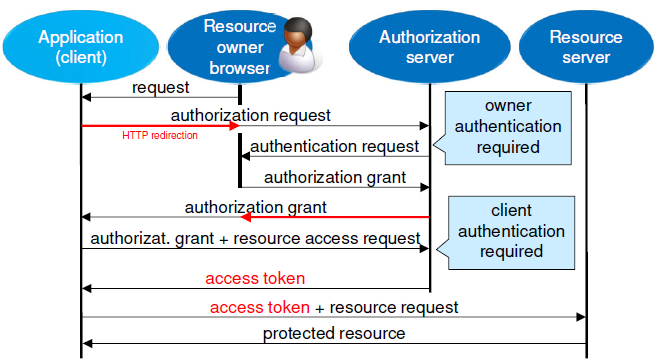
\includegraphics[scale=0.6]{29}
\end{center}

\subsection{OpenID Connect (OIDC)}

\begin{flushleft}
  \textbf{Uma camada de identificação em cima do OAuth 2.0}.
  OAuth 2.0 fornece a autenticação centralizada fundamental.
  Os recursos protegidos são os atributos da entidade,
  empacotados em \textbf{scopes}, os atributos são designados
  por (identity) \textbf{claims}.
\end{flushleft}

\pagebreak

\section{Armazenamento confiável}

\subsection{Problemas}

\begin{flushleft}
  \textbf{Os dispositivos de armazenamento desenvolvem falhas}
  \begin{itemize}
    \item As falhas devem ser minimizadas previnindo a perda de dados;
    \item As falhas acontecem de certeza, não podendo ser ignoradas;
  \end{itemize}

  \textbf{Acesso a discos pmecânicos é lento (hard disks (discos rigidos))}
  \begin{itemize}
    \item Tempo de acesso = tempo de translação + tempo de rotação;
    \item Mais informação $\rightarrow$ maior impacto na storage media;
  \end{itemize}

  \textbf{Solid State Devices (SSDs) têm um número limite de escritas}
  \begin{itemize}
    \item 2.000-3.000 escritas por MLC (2 bits por célula);
  \end{itemize}

  \textbf{Eventos especificos podem resultar na perda de dados}
  \begin{itemize}
    \item Incêndios, roubos, "picos de energia", inundações, erros
    humanos, ataques, \dots
  \end{itemize}

  \textbf{Pode ser necessário distribuir dados de uma forma inteligente}
  \begin{itemize}
    \item Maximizar a perfornance;
    \item Reduzir custos;
  \end{itemize}
\end{flushleft}

\subsection{Soluções}

\begin{flushleft}
  \textbf{Backups de dados}
  \begin{itemize}
    \item Local
    \item Remoto
  \end{itemize}

  \textbf{Armazenamento redundante}
  \begin{itemize}
    \item RAID (Redundant Array of Independent Disks)
    \item Other: ZFS
  \end{itemize}

  \textbf{Melhores dispositivos de armazenamento, ambientes com maior controlo}
  \begin{itemize}
    \item SLED (Single Large Expensive Disk)
    \item Enterprise Grade Devices
    \item Temperature and humidity controlled environments
  \end{itemize}

  \textbf{Infrastruturas dedicadas para armazenamento}
  \begin{itemize}
    \item Single policy control point
  \end{itemize}
\end{flushleft}

\pagebreak

\subsubsection{Backups}

\begin{flushleft}
  \textbf{Copiar os dados periodicamente}
  \begin{itemize}
    \item Snapshot do estado do armazenamento num momento específico;
    \item Cópias vão permitir recuperar versões anteriores de ficheiros;
    \item Podem ser encriptados;
  \end{itemize}

  \textbf{Full: Snapshot completo do volume de dados}
  \begin{itemize}
    \item Recuperação rápida;
    \item Requer muito espaço;
  \end{itemize}

  \textbf{Diferencial: Diferenças desde o último backup completo (full)}
  \begin{itemize}
    \item Recuperação mais lenta, mas também requer menos espaço;
    \item Este tipo de backups diariamente aumenta com o número de mudanças;
  \end{itemize}

  \textbf{Incremental: Diferenças desde o último backup}
  \begin{itemize}
    \item Recuperação ainda mais lenta;
    \item Requer reconstrução de todos os backups intermédios desde o úçtimo full backup;
    \item Mais eficiente em termos de espaço;
  \end{itemize}
\end{flushleft}

\textbf{Um backup não é um disco adicional com dados}, externo ou remoto. 
\textbf{Considera políticas, mecanismos e procedimentos para
fazer, manter e recuperar cópias dos mesmos dados}.
Deve resistir a situações especificas, deve ser usado apenas
em situações de emergência. É importante considerar
a cópia, armazenamento e recuperação!

\textbf{Legal framework implies a special care}:
\begin{itemize}
  \item Quando lidamos com dados pessoais;
  \item Impôr uma politica de retenção frequentemente, os backups
  devem expirar após um certo tempo;
\end{itemize}

\subsubsection{Backups - Types}

\begin{center}
  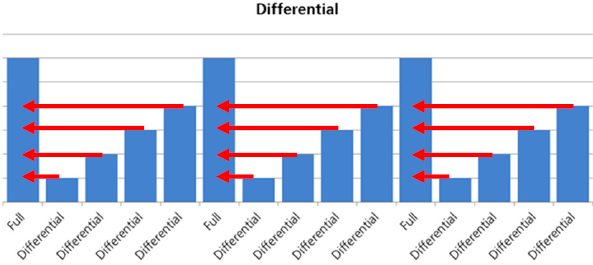
\includegraphics[scale=0.5]{30}
  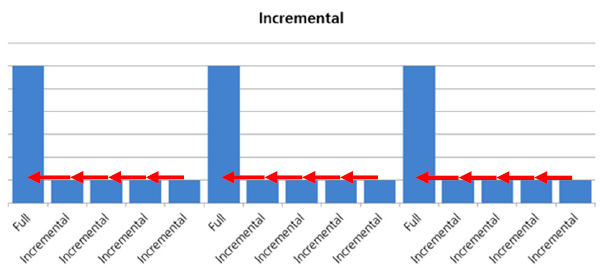
\includegraphics[scale=0.5]{31}
\end{center}

\pagebreak

\subsubsection{Backups: Compressão}

\begin{flushleft}
  \textbf{Usa algoritmos e soluções de compressão sem perdas}
  \begin{itemize}
    \item Ex: ZIP
  \end{itemize}

  \textbf{Copiar algumas partes da informação}
  \begin{itemize}
    \item Apenas ficheiros modificados;
  \end{itemize}

  \textbf{Deduplicação (deduplication)}
  \begin{itemize}
    \item Apenas guarda ficheiros/blocos únicos;
    \item Normalmente utiilizando full copy with deduplicação offline;
    \begin{itemize}
      \item De blocos do disco utilizando formatos de imagem especificos;
      \item De ficheiros utilizando hard links;
    \end{itemize}
  \end{itemize}
\end{flushleft}

\subsubsection{Backups: Níveis}

\begin{flushleft}
  \textbf{Aplicações}
  \begin{itemize}
    \item Extrair dados de aplicações (ex: mysqldump);
    \item Representar uma vista consistente da aplicação.
    Pode ser necessário bloquear o estado da aplicação (ex: mudanças na BD);
    \item Pode ser repetido para cada aplicação individual;
  \end{itemize}

  \textbf{Ficheiros}
  \begin{itemize}
    \item Copia de ficheiros individuais;
    \item Pode dar backup a qualquer sistema de ficheiro das aplicações;
    \item Estado pode ser inconsistente (ex: ficheiros abertos
    sem dados escritos, ou as aplicações mudam vários ficheiros de uma vez);  
  \end{itemize}

  \textbf{Sistema de Ficheiros}
  \begin{itemize}
    \item Funcionalidades internas fornecidas pelo sistema de ficheiros de cada individuo;
    \item Criação de snapshots periodicos com registos de todas as mudanças ou estado atual;
    \item Pode permitir a recuperação de ficheiros individuais, ou do sistema de ficheiros por completo;
  \end{itemize}

  \textbf{Blocos do Dispositivo}
  \begin{itemize}
    \item Copia de todos os blocos de um storage medium;
    \item Independente do sistema de ficheiros ou de sistema de operações me uso;
    \item Pode ser implementado pela Infrastrutura de Armazenamento (transparente e sem qualquer impacto para as aplicações);
  \end{itemize}
\end{flushleft}

\pagebreak

\subsubsection{Backups: Localização dos dados}

\begin{flushleft}
  \textbf{No mesmo volume ou o mesmo servidor}
  \begin{itemize}
    \item Permite aos utilziadores recuperar a informação rapidamente;
    \item Protege contra mudanças/deleções feitas pelos utilizadores;
    \item Pode não proteger contra mau funcionamento do hardware (ex: macOS Time Machine);
  \end{itemize}

  \textbf{Num sistema de localização na mesma infrastrutura}
  \begin{itemize}
    \item Também com acesso rápido;
    \item Protege contra falhas de armazenamento isoladas;
    \item Não protege os dados contra eventos como incêndios, inundações, roubo, \dots
    \item Ex: Most enterprise storage solutions, backuppc,
    TimeCapsule, Borg, Kopia
  \end{itemize}

  \textbf{Remoto (off-site)}
  \begin{itemize}
    \item Implementado para um sistema fora do datacenter local, serviço dedicado
    ou atraves da internet
    \begin{itemize}
      \item Ex: Amazon S3, ou servidores em datacenters dedicados;
      \item Encriptação se recomendado (ou obrigado) em caso de serviços externos;
    \end{itemize}

    \item Implementado com transporte seguro especializado (carro blindado transportando backups para um sitio seguro);
    \item Permite recuperação mesmo se eventos far-reaching aconteçam (ex: terrorismo, terremotos, \dots);
    \item Recuperação é mais lenta (limitada pela velocidade da rede ou do transporte fisico);
  \end{itemize}
\end{flushleft}

\subsection{Escolhendo Dispositivos de Armazenamento}

\begin{flushleft}
  \textbf{Different device grades: Enterprise vs Desktop}
  \begin{itemize}
    \item Diferentes qualidades de construção e funcionalidades de recuperação;
    \item Diferentes MTBF (Mean Time Between Failures)
    \begin{itemize}
      \item Enterprise HDD: 1.2M horas a 25ºC, trabalhando 24/7, 100\% use rate;
      \item Desktop HDD: 700K horas a 25ºC, trabalhando 8/5, 10-20\% use rate; 
    \end{itemize}
  \end{itemize}

  \textbf{Ajustar a cada use case}
  \begin{itemize}
    \item Write intensive vs read intensive;
    \item NAS vs Video vs Desktop vs Cold Storage vs Data Center
    (diferenças no consumo de energia, fiabilidade e performance);
  \end{itemize}

  \pagebreak

  \textbf{Ajustado a um nível especifico de performance}
  \begin{itemize}
    \item Tier 0: Melhor performance, baixa capacidade (PCIe NVME SLC SSD);
    \item Tier 1: Alguma performance, alta capacidade e disponibilidade (M2 SATA SSD);
    \item Tier 3: Baixa performance, alta capacidade, baico preço (SATA HDD);
  \end{itemize}
\end{flushleft}

\subsection{RAID (Redundant Array of Inexpensive Drives)}

\begin{flushleft}
  \textbf{Melhora a subrevivência da iniformação}
  \begin{itemize}
    \item Os dados são apenas perdidos depois de múltiplos dispositivos serem perdidos;
    \item O número de dispositivos perdidos é configurável;
  \end{itemize}

  \textbf{Baixo preço e solução eficiente}
  \begin{itemize}
    \item Pode usar hardware barato e de qualidade mais baixa;
    \item Podem melhorar a performance de leitura e escrita;
  \end{itemize}

  \textbf{RAID não substitui backups}
  \begin{itemize}
    \item Apenas tolera a falha de um número limitado de dispositivos;
    \item Não consegue lidar com erros humanos (mudificação/deleção de ficheiros);
  \end{itemize}

  \textbf{RAID pode até aumentar a probabilidade de falha}
  \begin{itemize}
    \item Uma vez que pode ser ajustado para obter melhor performance;
  \end{itemize}
\end{flushleft}

\subsubsection{RAID 0 (Striping)}

\begin{center}
  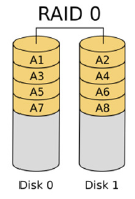
\includegraphics[scale=0.6]{32}
\end{center}

\begin{flushleft}
  \textbf{Objetivos:}
  \begin{itemize}
    \item Acelerar o acesso aos dados;
  \end{itemize}

  \textbf{Abordagem:}
  \begin{itemize}
    \item Acessar os discos em paralelo;
    \item \uline{Striping}
    \begin{itemize}
      \item Os dados são divididos em pequenos pedaços (stripes);
      \item Estes stripes são armazenados ao longo de todos os discos de uma forma distribuída;
    \end{itemize}
  \end{itemize}

  \pagebreak

  \textbf{Vantagens:}
  \begin{itemize}
    \item Pode acelerar a performance como fator do número de discos;
  \end{itemize}

  \textbf{Desvantagens:}
  \begin{itemize}
    \item Aumenta a probabilidade de perder dados
    (se \textbf{Pf} é a probabilidade de falha de um único disco,
    um volume RAID 0 com \textbf{N} discos tem uma probabilidade
    de falha de $1-(1-Pf)^N$);
    \item aumenta o número de dispositivos (pelo menos duplicando o número);
  \end{itemize}
\end{flushleft}

\subsubsection{RAID 1 (Mirroring)}

\begin{center}
  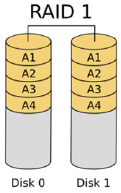
\includegraphics[scale=0.6]{33}
\end{center}

\begin{flushleft}
  \textbf{Objetivos:}
  \begin{itemize}
    \item Tolerância à falha de discos;
  \end{itemize}

  \textbf{Abordagem:}
  \begin{itemize}
    \item Duplicação dos dados (mirroring)
    \begin{itemize}
      \item Escrita sincronizada;
      \item Leitura desitribuida de qualquer disco com ou sem
      comparação com outro disco;
    \end{itemize}
  \end{itemize}

  \textbf{Vantagens:}
  \begin{itemize}
    \item Diminui a probabilidade de perda de dados
    (se \textbf{Pf} é a probabilidade de falha de um único disco,
    um volume RAID 1 com \textbf{N} discos tem uma probabilidade
    de falha de $Pf^N$);
  \end{itemize}

  \textbf{Desvantagens:}
  \begin{itemize}
    \item Armazenamento ineficiente (vai perder pelo menos 50\%
    da capacidade total, para 3 discos vai perder 66\% \dots $(N-1)/N$);
    \begin{itemize}
      \item Aumenta o número de dispositivos (pelo menos o dobro);
    \end{itemize}
  \end{itemize}
\end{flushleft}

\pagebreak

\subsubsection{RAID 0+1 e 1+0 (Nested)}

\begin{center}
  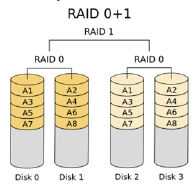
\includegraphics[scale=0.6]{34}
  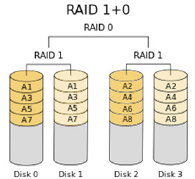
\includegraphics[scale=0.6]{35}
\end{center}

\begin{flushleft}
  \textbf{Objetivos:}
  \begin{itemize}
    \item Beneficios de RAID 0  (performance);
    \item Beneficios de RAID 1 (resiliência);
  \end{itemize}

  \textbf{Abordagem:}
  \begin{itemize}
    \item 0+1: Um volume RAID 1 utilizando volumes RAID 0 (mirroring of striped volumes);
    \item 1+0: RAID 0 sobre volumes RAID 1 (striping over mirrored volumes);
  \end{itemize}

  \textbf{Desvantagens:}
  \begin{itemize}
    \item Desperdicio da capacidade de armazenamento (pelo menos 50\%);
    \item Aumenta o número de dispositivos;
  \end{itemize}
\end{flushleft}

\subsubsection{RAID 4}

\end{document}